\chapter{\label{app:6-SCcompare}Bandgap deformation potential and supercell size}

The bandgap deformation is a function of Cartesian displacement, so that doubling the size of the supercell will scale the atomic displacements and bandgap change by a factor of $\frac{1}{\sqrt{2}}$ (Figure \ref{ch5scaling}).  % I don't really understand this!
Importantly, changing the supercell size scales the x-axis of the mode potential in the Schr\"{o}dinger solver so that the average bandgap for a given temperature, a physical observable, does not scale with supercell size.

\begin{figure}[]
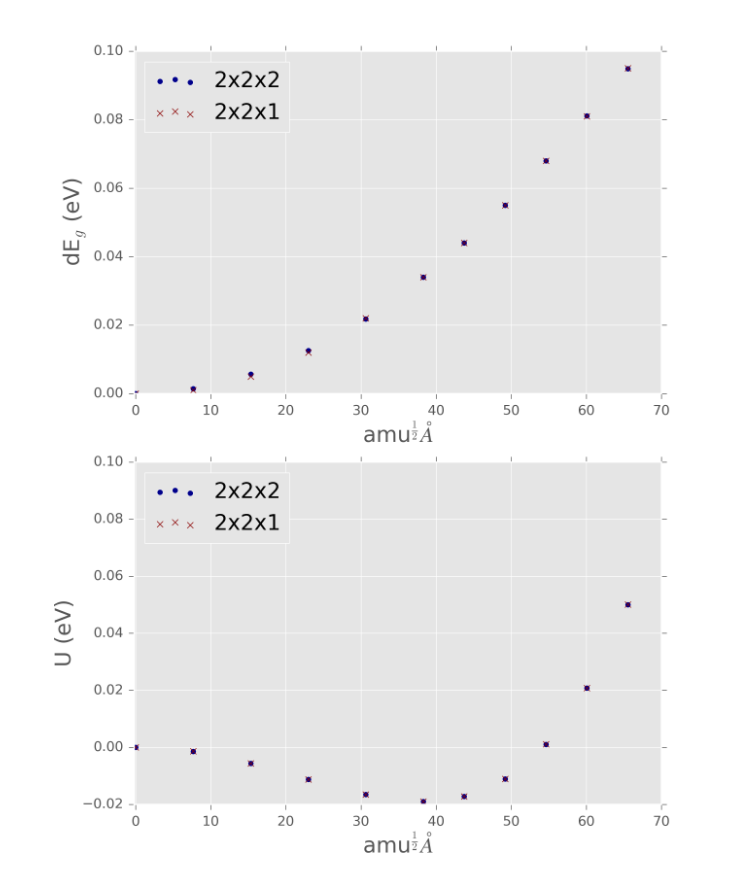
\includegraphics[width=0.6\textwidth]{figures/ch5/SCcompare.png} \centering 
\caption[Bandgap deformation potential and supercell size]{
Change in bandgap and the potential energy surface for two supercell sizes. To allow for comparison the x-axis values for the $2\times2\times1$ supercell have been scaled to match those of the $2\times2\times2$ supercell and the potential energy of the $2\times2\times1$ supercell has been doubled.  Differences in the calculated bandgap are of the order $10^{−4}\ \textrm{eV}$.
}
\end{figure}

